\subsection{PROPERTIES OF GROUPS ACTING PROPERLY}

PROPOSITION 3. If a topological group G operates properly on a topological space X, then the orbit space X/G is Hausdorff. If also G is Hausdorff, then X is Hausdorff.

Let \(C \subset X \times X\) be the graph of the equivalence relation \(R\) defined by \(G\) on \(X\) ; then \(C\) is the image of \(G \times X\) under the mapping \(\theta : (s, x) \to (x, s.x)\) . Since \(\theta\) is proper, \(C\) is closed in \(X \times X\) (Chapter I, § 10, no. 1, Proposition 1). Since the relation \(R\) is open (§ 2, no. 4, Lemma 2), it follows that \(X/G\) is Hausdorff (Chapter I, § 8, no. 3, Proposition 8).

Now suppose that G is Hausdorff. Then the mapping \(x \to (e, x)\) of X into \(G \times X\) is a homeomorphism of X onto a closed subspace of \(G \times X\) , and is therefore proper (Chapter I, § 10, no. 1, Proposition 2). If we compose this mapping with the mapping \((s, x) \to (x, s.x)\) of \(G \times X\) into \(X \times X\) , which by hypothesis is proper, we obtain a proper mapping of X into \(X \times X\) , namely the diagonal mapping \(x \to (x, x)\) . Hence the diagonal \(\Delta\) of \(X \times X\) is closed in X, and therefore X is Hausdorff.

PROPOSITION 4. Let G be a topological group operating properly on a topological space X, and let x be a point of X. Let G.x denote the orbit of x, and let \(K_{x}\) denote the stabilizer of x. Then:

\begin{enumerate}
\def\labelenumi{\alph{enumi})}
\item
  The mapping \(s \to s.x\) of \(G\) into \(X\) is proper.
\item
  \(\mathbf{K}_x\) is quasi-compact.
\item
  The canonical mapping of \(\mathbf{G} / \mathbf{K}_x\) onto \(\mathbf{G}.x\) is a homeomorphism.
\item
  The orbit G.x is closed in X.
\end{enumerate}

The inverse image of \(\{x\} \times X\) under \(\theta : (s, x) \to (x, s.x)\) is \(G \times \{x\}\) ; hence, by Proposition 3 of Chapter I, § 10, no. 1, the restriction of \(\theta\) to \(G \times \{x\}\) is a proper mapping of \(G \times \{x\}\) into \(\{x\} \times X\) , whence a) follows. Since \(K_x\) is the inverse image of \(x\) under \(s \to s.x\) , b) follows from Chapter I, § 10, no. 2, Theorem 1. c) and d) are consequences of a), by virtue of Chapter I, § 10, no. 1, Propositions 2 and 5 b).

Remark. Proposition 4 shows that if a topological group G operates properly on a homogeneous space G/H, then the subgroup H is quasi-compact (and therefore compact if G is Hausdorff). It can be shown that this is also a sufficient condition for G to operate properly on G/H (Exercise 3).

PROPOSITION 5. Let G (resp. G') be a topological group operating continuously on a topological space X (resp. X'). Let φ be a continuous homomorphism of G into \(\mathbf{G}'\) and let \(\psi\) be a continuous mapping of X into \(\mathbf{X}'\) compatible with \(\varphi\) ( \(\S 2\) , no. 4). Then:

\begin{enumerate}
\def\labelenumi{(\roman{enumi})}
\item
  If \(\varphi\) is surjective and \(\psi\) is surjective and proper, and if \(\mathbf{G}\) operates properly on \(\mathbf{X}\) , then \(\mathbf{G}'\) operates properly on \(\mathbf{X}'\) .
\item
  If \(\varphi\) is proper, if \(\mathbf{G}'\) operates properly on \(\mathbf{X}'\) and if \(\mathbf{X}\) is Hausdorff, then \(\mathbf{G}\) operates properly on \(\mathbf{X}\) .
\end{enumerate}

To prove (i), consider the commutative diagram

\[
\begin{array}{c c c c} \mathbf {G} & \times \mathbf {X} \xrightarrow {\theta} \mathbf {X} & \times \mathbf {X} \\ \alpha & \downarrow & & \downarrow \beta \\ \mathbf {G} ^ {\prime} & \times \mathbf {X} ^ {\prime} \xrightarrow {\theta^ {\prime}} \mathbf {X} ^ {\prime} & \times \mathbf {X} ^ {\prime} \end{array}
\]

where \(\alpha = \varphi \times \psi\) and \(\beta = \psi \times \psi\) . By hypothesis, \(\theta\) is proper; so is \(\beta\) {[}Chapter I, § 10, no. 1, Proposition 4a){]}; hence \(\beta \circ \theta = \theta' \circ \alpha\) is proper {[}Chapter I, § 10, no. 1, Proposition 5a){]}. Since \(\alpha\) is surjective it follows that \(\theta'\) is proper {[}Chapter I, § 10, no. 1, Proposition 5b){]}.

To prove (ii) consider an ultrafilter \(\mathfrak{U}\) on \(\mathbf{G} \times \mathbf{X}\) , such that the mappings

\[
(s, x) \rightarrow s. x \quad \text { and } \quad (s, x) \rightarrow x
\]

converge with respect to \(\mathfrak{U}\) to \(y_0\) and \(x_0\) respectively. It follows that \((s, x) \to \varphi(s). \psi(x)\) and \((s, x) \to \psi(x)\) converge with respect to \(\mathfrak{U}\) . Since \(\mathbf{G}'\) operates properly on \(\mathbf{X}'\) , this implies (no. 1) that \((s, x) \to \varphi(s)\) converges with respect to \(\mathfrak{U}\) to a point \(s_0' \in \mathbf{G}'\) . Since \(\varphi\) is proper, we deduce (Chapter I, § 10, no. 2, Theorem 1) that \((s, x) \to s\) converges with respect to \(\mathfrak{U}\) to a point \(s_0 \in \mathbf{G}\) . The uniqueness of the limit in \(\mathbf{X}\) then shows that \(y_0 = s_0 x_0\) , and hence that \(\mathbf{G}\) operates properly on \(\mathbf{X}\) (no. 1).

\subsection{GROUPS OPERATING FREELY ON A TOPOLOGICAL SPACE}

DEFINITION 2. Let G be a group operating on a set X. G is said to operate freely on X if the stabilizer of every element of X is \(\{e\}\) , in other words if the relations \(s.x = x, s \in G, x \in X\) imply s = e.

Example. Let G be a group and let H be a subgroup of G. Then H operates freely by (left or right) translations on G.

Let G be a group operating freely on a set X, let R be the equivalence relation defined by G on X, and let \(C \subset X \times X\) be the graph of R. If \((x, y) \in C\) , then there exists \(s \in G\) such that s.x = y; and s is unique, since \(s.x = s'.x\) implies \(s'^{-1}s.x = x\) , and therefore \(s'^{-1}s = e\) (as G operates freely). If we make correspond to \((x, y) \in C\) the unique \(s \in G\) such that s.x = y, we define a mapping \(\varphi: C \to G\) , which we shall call the canonical mapping of C into G. With this notation:

PROPOSITION 6. Let G be a topological group operating continuously on a topological space X, and suppose that G operates freely on X. Then G operates properly on X if and only if the following condition is satisfied:

(FP) The graph C of the equivalence relation defined by G is closed in \(X \times X\) , and the canonical mapping \(\varphi: C \rightarrow G\) is continuous.

The set C is the image of the mapping \(\theta: (s, x) \to (x, s.x)\) of \(\mathbf{G} \times \mathbf{X}\) into \(\mathbf{X} \times \mathbf{X}\) . We know (Chapter I, § 10, no. 1, Proposition 2) that \(\theta\) is proper if and only if C is closed in \(\mathbf{X} \times \mathbf{X}\) and (if \(\theta'\) denotes the mapping \(\theta\) considered as a mapping of \(\mathbf{G} \times \mathbf{X}\) into C) \(\theta'\) is a homeomorphism. Now the hypothesis implies that \(\theta'\) is bijective and that its inverse is the mapping \((x, y) \to (\varphi(x, y), x)\) . Hence \(\theta'\) is a homeomorphism if and only if \(\varphi\) is continuous.

\subsection{LOCALLY COMPACT GROUPS OPERATING PROPERLY}

PROPOSITION 7. Let G be a locally compact group operating continuously on a Hausdorff space X. Then G operates properly on X if and only if, for each pair of points x, y of X, there is a neighbourhood \(V_{x}\) of x and a neighbourhood \(V_{y}\) of y such that the set K of all \(s \in G\) for which \(s \cdot V_{x} \cap V_{y} \neq \emptyset\) is relatively compact in G.

Let F be the compact space obtained by adjoining a point at infinity \(\omega\) to G, and let \(\Gamma\) be the graph of \(\rho: (s, x) \to s.x\) considered as a subset of \(F \times X \times X\) . Let us show that if the restriction of \(pr_{23}\) to \(\Gamma\) is proper, then \(\Gamma\) is closed in \(F \times X \times X\) . Indeed, this hypothesis implies that the map \(u: (t, s, x, y) \to (t, x, y)\) of \(F \times \Gamma\) into \(F \times X \times X\) is closed. If \(\Gamma'\) is the set of points \((s, s)\) in \(F \times G\) , where \(s \in G\) , then \(\Gamma'\) is closed in \(F \times G\) , since it is the graph of the canonical injection \(G \to F\) (Chapter I, §8, no. I, Corollary 2 to Proposition 2); hence the intersection \((\Gamma' \times X \times X) \cap (F \times \Gamma)\) is closed in \(F \times \Gamma\) , and it is immediately seen that its image under u is the set \(\Gamma\) considered as a subset of \(F \times X \times X\) ; hence \(\Gamma\) is closed in \(F \times X \times X\) . Now, we have \((\{\omega\} \times X \times X) \cap \Gamma = \emptyset\) . From the definition of F, therefore, for every point \((x, y) \in X \times X\) there is a neighbourhood W of \((x, y)\) in \(X \times X\) and a compact subset K of G such that

\[
((\mathbf {G} - \mathbf {K}) \times \mathbf {W}) \cap \Gamma ;
\]

is empty; and since we may take W to be a neighbourhood \(V_{x} \times V_{y}\) , where \(V_{x}\) and \(V_{y}\) are neighbourhoods of x and y respectively in X, the statement ``((G - K) × W) ∩ Γ = ∅'' becomes ``if s∉K, then s.Vx∩Vy=∅''. We have thus proved the necessity of the condition stated in the proposition. Conversely, suppose this condition is satisfied; let A be a set filtered by an ultrafilter \(\mathfrak{F}\), and let \(\alpha \to (s_{\alpha}, x_{\alpha})\) be a mapping of A into \(G \times X\) such that \(\lim_{\mathfrak{F}} x_{\alpha} = x\) and \(\lim_{\mathfrak{F}} s_{\alpha}\cdot x_{\alpha} = y\). Suppose that K, Vx and Vy satisfy the condition of the proposition. By hypothesis there is a set \(M \in \mathfrak{F}\) such that if \(\alpha \in M\) then \(x_{\alpha} \in V_{x}\) and \(s_{\alpha}\cdot x_{\alpha} \in V_{y}\), hence \(s_{\alpha} \in K\). This shows that \(\alpha \to s_{\alpha}\) converges with respect to \(\mathfrak{F}\), and the proof is complete.

If G is compact, the condition of Proposition 7 is trivially satisfied; we thus retrieve Proposition 2a).

Proposition 7 shows in particular that a discrete group G, operating continuously on a Hausdorff space X, operates properly on X if and only if, for each pair \((x, y)\) of points of X, there is a neighbourhood \(V_{x}\) of x and a neighbourhood \(V_{y}\) of y such that the set of points \(s \in G\) for which \(s \cdot V_{x} \cap V_{y} \neq \emptyset\) is finite.

PROPOSITION 8. Let G be a discrete group operating properly on a Hausdorff space X. Let x be a point of X and let \(K_{x}\) be the stabilizer of x. Then:

\begin{enumerate}
\def\labelenumi{\alph{enumi})}
\item
  The subgroup \(K_{x}\) is finite and there is an open set \(U \subset X\) , containing x, which is stable under \(K_{x}\) , and on which the equivalence relation induced by the relation defined by G is the equivalence relation defined by \(K_{x}\) .
\item
  The canonical mapping \(\mathbf{U} / \mathbf{K}_x\to \mathbf{X} / \mathbf{G}\) is a homeomorphism of \(\mathbf{U} / \mathbf{K}_x\) onto an open neighbourhood of the class of \(x\) in \(\mathbf{X} / \mathbf{G}\) .
\end{enumerate}

By Proposition 7, \(\mathbf{K}_x\) is finite. To construct an open set \(\mathbf{U}\) which satisfies the required conditions, notice first that by Proposition 7 there is an open set \(\mathrm{U}_0\) containing \(x\) and such that the set \(\mathbf{K}\) of \(s \in \mathbf{G}\) for which \(s. \mathrm{U}_0 \cap \mathrm{U}_0 \neq \emptyset\) is finite. Clearly \(\mathbf{K}_x \subset \mathbf{K}\) ; let \(s_1, \ldots, s_n\) be the elements of \(\mathbf{K} - \mathbf{K}_x\) . If we put \(x_i = s_i.x\) ( \(1 \leqslant i \leqslant n\) ), then \(x_i \neq x\) for each \(i\) ; since \(\mathbf{X}\) is Hausdorff, there is for each index \(i\) an open neighbourhood \(\mathrm{V}_i\) of \(x\) and an open neighbourhood \(\mathrm{V}_i'\) of \(s_i.x\) such that \(\mathrm{V}_i \cap \mathrm{V}_i' = \emptyset\) . Let \(\mathrm{U}_i = \mathrm{V}_i \cap s_i^{-1}. \mathrm{V}_i'\) ; then \(\mathrm{U}_i\) is clearly open and contains \(x\) , and we have \(\mathrm{U}_i \cap s_i. \mathrm{U}_i \subset \mathrm{V}_i \cap \mathrm{V}_i' = \emptyset\) . Let \(\mathrm{U}' = \mathrm{U}_0 \cap \mathrm{U}_1 \cap \ldots \cap \mathrm{U}_n\) ; \(\mathrm{U}'\) is open, contains \(x\) and is such that \(\mathrm{U}' \cap s. \mathrm{U}' = \emptyset\) for \(s \notin \mathbf{K}_x\) . Putting \(\mathrm{U} = \bigcap_{t \in \mathbf{K}_x} t. \mathrm{U}'\) we finally obtain an open set, stable under \(\mathbf{K}_x\) , containing \(x\) and such that \(\mathrm{U} \cap s. \mathrm{U} = \emptyset\) for \(s \notin \mathbf{K}_x\) : \(\mathrm{U}\) is the open set required.

The fact that the canonical mapping \(\mathbf{U} / \mathbf{K}_x\to \mathbf{X} / \mathbf{G}\) is a homeomorphism of \(\mathbf{U} / \mathbf{K}_x\) onto an open set in \(\mathbf{X} / \mathbf{G}\) follows from Chapter I, § 5, no. 2, Proposition 4, since \(\mathbf{U}\) is open and the equivalence relation defined by \(\mathbf{G}\) is open (§ 2, no. 4, Lemma 2).

COROLLARY. If we suppose in addition that \(K_{x}=\{e\}\) , then the point x has an open neighbourhood U such that the restriction to U of the canonical mapping \(X\to X/G\) is a homeomorphism of U onto an open subset of X/G.

\subsection{GROUPS OPERATING CONTINUOUSLY ON A LOCALLY COMPACT SPACE}

PROPOSITION 9. Let G be a topological group operating continuously on a locally compact space X. Then if X/G is Hausdorff it is locally compact.

Since the equivalence relation on X defined by G is open (§ 2, no. 4, Lemma 2), the proposition results from Chapter I, § 10, no. 4, Proposition 10.

PROPOSITION 10. Let G be a topological group operating continuously on a locally compact space X, and suppose that X/G is Hausdorff. Let \(\varphi\) be the canonical mapping of X onto X/G. Then if K' is any compact subset of X/G, there is a compact subset K of X such that \(\varphi(K) = K'\) .

Since the equivalence relation defined by G is open (§ 2, no. 4, Lemma 2), the proposition is a particular case of Proposition 10 of Chapter I, § 10, no. 4.

PROPOSITION 11. Let G be a Hausdorff topological group operating properly on a non-empty space X. If X is compact (resp. locally compact) then so are G and X/G.

By hypothesis, the mapping \(\theta : (s, x) \to (x, s.x)\) of \(G \times X\) into \(X \times X\) is proper; if \(X \times X\) is compact (resp. locally compact) then the Corollary to Proposition 9 of Chapter I, § 10, no. 4 shows that \(G \times X\) is also compact (resp. locally compact), and therefore so is \(G\) since \(X \neq \emptyset\) . Since \(X/G\) is Hausdorff (no. 2, Proposition 3), the compactness (resp. local compactness) of \(X\) implies the compactness (resp. local compactness) of \(X/G\) {[}Chapter I, § 10, no. 4, Proposition 8 (resp. Proposition 9){]} (see § 2, Exercise 29).

We shall now give criteria which allow us to assert that a Hausdorff topological group G operates properly on a locally compact space X. For each pair of subsets K, L of X we denote by P(K, L) the set of all \(s \in G\) such that \(s \cdot K \cap L \neq \emptyset\) .

THEOREM 1. Let G be a Hausdorff topological group which operates continuously on a topological space X. Let K be a compact subset of X and let L be a closed subset of X. Then:

\begin{enumerate}
\def\labelenumi{\alph{enumi})}
\item
  The set \(\mathbf{P}(\mathbf{K},\mathbf{L})\) is closed in \(\mathbf{G}\) .
\item
  If G operates properly on X and if L is compact, then P(K, L) is compact.
\item
  Conversely, if X is locally compact and if, for each pair K, L of compact subsets of X, P(K, L) is relatively compact in G {[}and therefore compact by a){]}; then G operates properly on X (and if X is not empty, G is locally compact by Proposition 11).
\end{enumerate}

The mapping \((s, x) \to s.x\) of \(G \times K\) into X is continuous, and the inverse image \(L'\) of L under this mapping is therefore closed. Since K is compact, the projection \(pr_{1}: G \times K \to G\) is proper (Chapter I, § 10, no. 2, Corollary 5 of Theorem 1) and the image of \(L'\) under \(pr_{1}\) is therefore closed. This image is \(P(K, L)\) , hence a) is proved.

To prove b): X is Hausdorff (no. 2, Proposition 3). By hypothesis the mapping \(\theta: (s, x) \to (x, s.x)\) of \(G \times X\) into \(X \times X\) is proper; since \(K \times L\) is compact, so is \(\theta^{-1}(K \times L)\) since \(X\) is Hausdorff (Chapter I, § 10, no. 2, Proposition 6). Hence the projection \(P(K, L)\) of \(\theta^{-1}(K \times L)\) into \(G\) is a compact set.

To prove c): since \(K \times L\) is closed in \(X \times X\) , it follows that \(\theta^{-1}(K \times L)\) is closed in \(P(K, L) \times K\) and is therefore compact under the hypotheses of c). Since every compact subset of \(X \times X\) is contained in a compact subset of the form \(K \times L\) , it follows that the inverse image of any compact subset of \(X \times X\) under \(\theta\) is compact, and since \(X \times X\) is locally compact, this shows that \(\theta\) is proper (Chapter I, § 10, no. 3, Proposition 7) {[}see Chapter IV, § 1, Exercise 4c){]}.

Remark. Clearly, we have \(\mathrm{P}(\mathrm{K},\mathrm{L})\subset\mathrm{P}(\mathrm{K}\cup\mathrm{L},\mathrm{K}\cup\mathrm{L})\) ; therefore for G to operate properly on a locally compact space X, it is sufficient that, for each compact subset K of X, the set \(\mathrm{P}(\mathrm{K},\mathrm{K})\) is relatively compact in G. In particular, a discrete group G operates properly on a locally compact space X if and only if, for each compact subset K of X, the set of \(s\in G\) such that \(s.K\cap K\neq\emptyset\) is finite.

Example. * Let X be a complex analytic manifold, analytically isomorphic to a bounded open subset of \(\mathbf{C}^n\) , and let G be the group of analytic automorphisms of X. The topology of compact convergence is compatible with the group structure of G, and it can be shown that G operates properly on X. In particular, every discrete subgroup of G operates properly on X.

Take for example X to be the upper half-plane \(\mathfrak{J}(z)>0\) , which is analytically isomorphic to an open disc in C. Then G is the group of all transformations \(z\to (az+b)/(cz+d)\) , where \(a,b,c,d\) are real and \(ad-bc\neq0\) . The subgroup H of G which consists of all such transformations for which \(a,b,c,d\) are integers and \(ad-bc=1\) is a discrete subgroup of G, called the modular group. By what has been said above, it operates properly on the upper half-plane \(\mathfrak{J}(z)>0\) . *

PROPOSITION 12. Let G be a Hausdorff topological group which operates continuously on a topological space X. Let K be a compact subset of X, and let \(\rho_{K}\) be the mapping \((s, x) \to s.x\) of \(G \times K\) into X. Then:

\begin{enumerate}
\def\labelenumi{\alph{enumi})}
\item
  If G operates properly on X, \(\rho_{\mathbf{K}}\) is proper.
\item
  If X is locally compact and \(\rho_{K}\) is proper for each compact subset K of X, G operates properly on X.
\end{enumerate}

The mapping \(\rho_{\mathbf{K}}\) factorizes as \(\mathbf{G} \times \mathbf{K} \xrightarrow{\theta_{\mathbf{K}}} \mathbf{K} \times \mathbf{X} \xrightarrow{\mathrm{pr}_2} \mathbf{X}\) , where \(\theta_{\mathbf{K}}\) is the restriction to \(\mathbf{G} \times \mathbf{K}\) of the mapping \(\theta: (s, x) \to (x, s.x)\) of \(\mathbf{G} \times \mathbf{X}\) into \(\mathbf{X} \times \mathbf{X}\) . Since \(\theta^{-1}(\mathbf{K} \times \mathbf{X}) = \mathbf{G} \times \mathbf{K}\) , \(\theta_{\mathbf{K}}\) is proper if \(\theta\) is proper (Chapter I, § 10, no. 1, Proposition 3). On the other hand, since \(\mathbf{K}\) is compact, the projection \(\mathrm{pr}_2: \mathbf{K} \times \mathbf{X} \to \mathbf{X}\) is proper (Chapter I, § 10, no. 2, Theorem 1, Corollary 5), hence \(\rho_{\mathbf{K}}\) is proper (ibid., no. 1, Proposition 5).

Suppose conversely that \(\rho_{\mathbf{K}}\) is proper for each compact \(\mathbf{K} \subset \mathbf{X}\) . If \(\mathbf{L}\) is a compact subset of \(\mathbf{X}\) , then \(\rho_{\mathbf{K}}^{-1}(\mathbf{L})\) is a compact subset of \(\mathbf{G} \times \mathbf{K}\) , whose projection into \(\mathbf{G}\) is \(\mathrm{P}(\mathbf{K}, \mathbf{L})\) ; therefore \(\mathrm{P}(\mathbf{K}, \mathbf{L})\) is compact. Hence if \(\mathbf{X}\) is locally compact it follows from Theorem 1 that \(\mathbf{G}\) operates properly on \(\mathbf{X}\) .

COROLLARY. Let G be a Hausdorff topological group operating properly on a topological space X. If K is any compact subset of X and if F is any closed subset of G, then F.K is closed in X.

This follows from Proposition 12 and from Chapter I, § 10, no. 1, Proposition 1.

\subsection{LOCALLY COMPACT HOMOGENEOUS SPACES}

PROPOSITION 13. Let G be a locally compact group and let H be a closed subgroup of G. Then the homogeneous space G/H is locally compact and paracompact.

Since G/H is Hausdorff (§ 2, no. 5, Proposition 13) it is locally compact, by Proposition 9 of no. 5 applied to H operating on G on the right. Thus it remains to show that G/H is paracompact. Let V be a symmetric compact neighbourhood of e in G, and let \(G_{0}=V^{\infty}\) be the subgroup of G generated by V. \(G_{0}\) is open (§ 2, no. 1, Corollary to Proposition 4) and operates continuously on G/H (§ 2, no. 5, Proposition 12). If we can show that each of the orbits \(G_{0}.z\) ( \(z\in G/H\) ) is an open subset of G/H and a countable union of compact sets, then it will follow that G/H is the topological sum of the distinct orbits \(G_{0}.z\) and is therefore paracompact (Chapter I, § 9, no. 10, Theorem 5). That \(\mathbf{G}_0.z\) is open in G/H follows from the facts that \(\mathbf{G}_0\) is open in G and the equivalence relation \(x^{-1}y\in H\) is open (§ 2, no. 4, Lemma 2). On the other hand, \(\mathbf{G}_0.z\) is the union of the sets \(\mathbf{V}^n.z\) ( \(n\geqslant 1\) ), and since \(\mathbf{V}^n\) is compact in G and G/H is Hausdorff, \(\mathbf{V}^n.z\) is compact. This completes the proof.

PROPOSITION 14. In a locally compact group G, the identity component C is the intersection of the open subgroups of G.

C is a closed normal subgroup of G (§ 2, no. 2, Proposition 7), and hence G/C is locally compact (Proposition 13) and totally disconnected (Chapter I, § 11, no. 5, Proposition 9). Since the inverse image of an open subgroup of G/C, under the canonical mapping of G onto G/C, is an open subgroup of G containing C, we see that we can restrict ourselves to proving the proposition for the group G/C. In other words, we may assume that G is totally disconnected. We know then (Chapter II, § 4, no. 4, Corollary to Proposition 6) that every compact neighbourhood V of e contains a neighbourhood U of e which is both open and closed. Since U is compact and \(B = \complement U\) is closed, there is a symmetric open neighbourhood W of e such that W ⊂ U and UW ∩ BW = ∅ (§ 3, no. 1 and Chapter II, § 4, no. 3, Proposition 4), and a fortiori UW ⊂ U. By induction on n it follows that \(W^n \subset U\) for every integer \(n > 0\). Hence the subgroup \(W^\infty = \bigcup_{n > 0} W^n\), generated by W, is contained in U; but \(W^\infty\) is open in G (§ 2, no. 1, Corollary to Proposition 4). This completes the proof.

We have also proved :

COROLLARY 1. If G is a totally disconnected locally compact group, then every neighbourhood of e in G contains an open subgroup of G.

COROLLARY 2. A locally compact group is connected if it is generated by each neighbourhood of the identity element.

COROLLARY 3. Let G be a locally compact group, let H be a closed subgroup of G, and let \(\varphi\) be the canonical mapping of G onto G/H. Then the components of G/H are the closures of the images under \(\varphi\) of the components of G.

Let C be the identity component of G. The components of G are the sets sC, where \(s \in G\) (§ 2, no. 2, Proposition 7); \(\varphi(sC)\) is clearly connected, hence so is \(\overline{\varphi(sC)}\) (Chapter I, § 11, no. 1, Proposition 1). But \(\varphi(sC) = \varphi(sCH)\) , and since sCH is saturated with respect to the equivalence relation defined by H, and since this equivalence relation is open

(§ 2, no. 4, Lemma 2), we have \(\overline{\varphi(s\mathbf{CH})} = \varphi(\overline{s\mathbf{CH}}) = \varphi(s.\overline{\mathbf{CH}})\) (Chapter I, § 5, no. 3, Proposition 7).

Put L = CH. L is a closed subgroup of G which contains C and H; hence to prove that the sets \(\varphi(s.L) = s.\varphi(L)\) are the components of G/H it is enough to show that the quotient space of G/H by the equivalence relation whose classes are the sets \(s.\varphi(L)\) is totally disconnected. Now this quotient space is homeomorphic to the homogeneous space G/L (Chapter I, § 3, no. 4, Proposition 7); we are thus reduced to proving that when \(C \subset H\) , G/H is totally disconnected. Since G/H may be identified with \((\mathrm{G/C})/(\mathrm{H/C})\) (§ 2, no. 7, Proposition 22), we may even assume that G itself is totally disconnected. Every neighbourhood of \(\varphi(e)\) in G/H contains a neighbourhood of the form \(\varphi(V)\) , where V is a neighbourhood of e in G, and therefore (Corollary 1) contains a neighbourhood of the form \(\varphi(K)\) , where K is a compact open subgroup of G. \(\varphi(K)\) is therefore both open and closed in G/H, and this shows that the component of \(\varphi(e)\) in G/H consists of \(\varphi(e)\) alone. By translation, the same is true for the component of every point of G/H, and the corollary is proved.

\section{INFINITE SUMS IN COMMUTATIVE GROUPS}

\subsection{SUMMABLE FAMILIES IN A COMMUTATIVE GROUP}

In this section we shall be concerned only with Hausdorff commutative topological groups, whose law of composition is written additively. Only the most important results will be translated into multiplicative notation.

Let \(\mathbf{G}\) be a Hausdorff commutative group, let \(\mathbf{I}\) be any index set and let \((x_{i})_{i\in \mathbf{I}}\) be a family of points of \(\mathbf{G}\) , indexed by \(\mathbf{I}\) . With each finite subset \(\mathbf{J}\) of \(\mathbf{I}\) we associate the element \(s_{\mathbf{J}} = \sum_{i\in \mathbf{J}}x_i\) of \(\mathbf{G}\) , which

we call the finite partial sum of the family \((x_{i})_{i\in I}\) , corresponding to the set \(J\) . If \(\mathfrak{F}(I)\) denotes the set of finite subsets of \(I\) , we have thus a mapping \(J\to s_J\) of \(\mathfrak{F}(I)\) into \(G\) . Now \(\mathfrak{F}(I)\) is a directed set with respect to the relation \(\subset\) ; for if \(J\) and \(J'\) are two elements of \(\mathfrak{F}(I)\) , then \(J\subset J\cup J'\) and \(J'\subset J\cup J'\) , and \(J\cup J'\) is a finite subset of \(I\) . Let \(\Phi\) be the section filter of the directed set \(\mathfrak{F}(I)\) (Chapter I, § 6, no. 3).

DEFINITION 1. Let \((x_{i})_{i\in I}\) be a family of points of a Hausdorff commutative group G; let \(\mathfrak{F}(I)\) be the set of finite subsets of the index set \(I\) , and for each finite subset \(J\) of \(I\) , let \(s_J\) be the sum of those \(x_{i}\) such that \(i\in J\) . The family \((x_{i})_{i\in I}\) is said to be summable if the mapping \(J\to s_J\) has a limit with respect to the section filter \(\Phi\) of the set \(\mathfrak{F}(I)\) directed by the relation \(\subset\) ; this limit is then said to be the sum of the family \((x_{i})_{i\in I}\) and is denoted by \(\sum_{i\in I}x_{i}\) (or simply \(\sum x_{i}\) , or even \(\sum x_{i}\) , when there is no risk of ambiguity).

Definition 1 is equivalent to the following: the family \((x_{i})\) is summable and its sum is \(s\) if, for each neighbourhood \(\mathbf{V}\) of the origin in \(\mathbf{G}\) , there is a finite subset \(\mathbf{J}_0\) of \(\mathbf{I}\) such that for each finite subset \(\mathbf{J} \supset \mathbf{J}_0\) of \(\mathbf{I}\) we have \(s_{\mathbf{J}} \in s + \mathbf{V}\) .

If G is written multiplicatively, and if we put \(p_{J} = \prod_{i \in J} x_i\) for each finite subset J of I, the family \((x_i)\) will be said to be multipliable if the mapping \(J \to p_J\) has a limit with respect to the filter \(\Phi\) ; this limit is called the product of the family \((x_i)\) , and is denoted by \(\prod_{i \in I} x_i\) .

Remarks. 1) When I is finite, Definition 1 reduces to the ordinary definition of the sum of a finite family. More generally, if I is arbitrary and \(x_{i} = 0\) except when the index \(i\) belongs to a finite subset J of I, then the sum \(\sum_{i \in I} x_{i}\) is equal to \(\sum_{i \in J} x_{i}\) .

\begin{enumerate}
\def\labelenumi{\arabic{enumi})}
\setcounter{enumi}{1}
\item
  The definition of a summable family does not involve any ordering of the index set I, and we may therefore say that the notion of a sum thus defined is commutative. More precisely, we have the following property: let \((x_{t})_{t\in \mathbf{I}}\) be a summable family and let \(\varphi\) be a bijective mapping of an index set K onto the set I; then if we put \(y_{x} = x_{\varphi (x)}\) , the family \((y_{x})_{x\in \mathbb{K}}\) is summable and has the same sum as \((x_{t})\) . For if \(s = \sum_{i\in I}x_i\) , and if \(\sum_{i\in J}x_i\in s + V\) for every finite subset J containing the finite subset \(J_0\) , then we shall have \(\sum_{x\in L}y_x\in s + V\) for every finite subset L of K containing \(\varphi^{-1}(J_0)\) .
\item
  Definition 1 applies, more generally, to every family of points in a Hausdorff topological space X on which has been defined an associative and commutative law of composition, written additively; for it does not make use of the axioms of topological groups.
\end{enumerate}

\subsection{CAUCHY'S CRITERION}

Let \((x_{t})_{t\in I}\) be a summable family in \(G\) . Then for each neighbourhood \(V\) of the origin in \(G\) there is a finite subset \(J_{0}\) of \(I\) such that,

for each finite subset K of I which does not meet \(J_{0}\) , we have \(s_{K} \in V\) . For \(J = J_{0} \cup K\) is an arbitrary finite subset containing \(J_{0}\) ; let \(s = \sum x_{i}\) and let W be a symmetric neighbourhood of o such that \(W + W \subset V\) ; then, by Definition 1, we may choose \(J_{0}\) such that \(s_{J} \in s + W\) and \(s_{J_{0}} \in s + W\) , which means that \(s_{K} = s_{J} - s_{J_{0}} \in W + W \subset V\) .

Conversely, suppose that the family \((x_{i})\) has this property. Then the image of the filter \(\Phi\) , under the mapping \(J \to s_{J}\) , is a Cauchy filter base in G. For if J is a finite subset containing \(J_{0}\) , and if K denotes \(J \cap \complement J_{0}\) , then \(K \cap J_{0} = \emptyset\) and \(s_{K} = s_{J} - s_{J_{0}}\) , so that \(s_{J} \in s_{J_{0}} + V\) . If \(J'\) is another finite subset containing \(J_{0}\) , then \(s_{J} - s_{J'} \in V + V\) , and the result follows. Consequently:

THEOREM 1 (Cauchy's criterion). In a Hausdorff commutative group G, in order that a family \((x_{t})_{t\in I}\) should be summable it is necessary that, for each neighbourhood V of the origin in G, there is a finite subset \(J_0\) of I such that \(\sum_{i\in K}x_i\in V\) for all finite subsets K of I which do not meet \(J_0\) . This necessary condition is also sufficient if G is complete.

Thus by taking away a (sufficiently large) finite number of terms from the family \((x_{i})\) , every finite partial sum of the surviving subfamily has to be as close to o as we please.

An immediate consequence of the first part of Theorem 1 is the following proposition:

PROPOSITION 1. If the family \((x_{t})\) is summable, then every neighbourhood of o contains all the \(x_{t}\) except for a finite subfamily (in other words, if I is infinite, we have \(\lim x_{t} = 0\) with respect to the filter of complements of finite subsets of I).

\pandocbounded{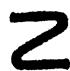
\includegraphics[keepaspectratio]{images/part002_cfff7d82.jpg}}

This necessary condition for a family \((x_{i})\) to be summable is by no means sufficient in general, even if \(G\) is complete; we shall see many examples later (see Chapter IV, § 7).

COROLLARY. Let \((x_{t})_{t\in I}\) be a summable family in a commutative group whose identity element has a countable fundamental system of neighbourhoods. Then the set of indices \(\iota\) such that \(x_{\iota}\neq 0\) is countable.

Let \((\mathbf{V}_{n})\) be a countable fundamental system of neighbourhoods of 0. If \(\mathbf{H}_{n}\) is the set of all indices i such that \(x_{i} \notin \mathbf{V}_{n}\) , then the set H of indices i such that \(x_{i} \neq 0\) is the union of the sets \(\mathbf{H}_{n}\) , and each of the \(\mathbf{H}_{n}\) is finite by Proposition 1.

This corollary is no longer necessarily valid if we do not assume that the origin has a countable fundamental system of neighbourhoods. * Consider, for example, the product group \(\mathbf{R}^{\mathbb{R}}\) {[}the additive group of all finite real-valued functions of a real variable, with the topology of pointwise convergence (cf.~Chapter X, § 1, no. 3){]}, and let \(f_{a}\) be the element of \(\mathbf{R}\) such that \(f_{a}(a)=1\) and \(f_{a}(x)=0\) if \(x\neq a\) ; then the family \((f_{a})_{a\in\mathbb{R}}\) is summable and its sum is the function whose value at each point of \(\mathbf{R}\) is 1. *

Remark. When G is written multiplicatively, Cauchy's criterion takes the following form: for the family \((x_{i})_{i\in I}\) to be multipliable it is necessary that, for each neighbourhood V of the identity element, there should exist a finite subset \(J_{0}\) of I such that, for each finite subset K of I which does not meet \(J_{0}\) , we have \(\prod_{i\in K}x_{i}\in V\) ; and this condition is sufficient provided that G is complete. We deduce that if I is infinite and \((x_{i})\) is multipliable, then \(\lim x_{i}=1\) with respect to the filter of complements of finite subsets of I; if in addition the identity element has a countable fundamental system of neighbourhoods, then the set of indices i such that \(x_{i}\neq1\) is countable.

\subsection{PARTIAL SUMS; ASSOCIATIVITY}

PROPOSITION 2. In a complete group G, every subfamily of a summable family is summable.

For if Cauchy's criterion is satisfied by a family \((x_{i})_{i\in I}\) , then it is trivially satisfied by every subfamily.

If \((x_{i})_{i\in I}\) is summable, it follows therefore that the sum \(\sum_{i\in J}x_{i}\) is defined for every subset \(J\) of \(I\) , finite or not: it is again called the partial sum of the family \((x_{i})\) , corresponding to the subset \(J\) of the index set. The set of partial sums of a summable family is evidently contained in the closure of the set of finite partial sums.

THEOREM 2 (Associativity of the sum). Let \((x_{i})_{i\in I}\) be a summable family in a complete group \(\mathbf{G}\) , and let \((I_{\lambda})_{\lambda \in L}\) be any partition of \(\mathbf{I}\) . If \(s_{\lambda}\) denotes \(\sum_{i\in I_{\lambda}}x_{i}\) , then the family \((s_{\lambda})_{\lambda \in L}\) is summable and has the same sum as the family \((x_{i})_{i\in I}\) .

Let \(s = \sum_{i \in I} x_i\) , and let \(V\) be any closed neighbourhood of 0 in \(G\) . Then there is a finite subset \(J_0\) of \(I\) such that, for each finite subset \(J\) of \(I\) which contains \(J_0\) , we have \(\sum_{i \in J} x_i \in s + V\) . Let \(K_0\) be the subset of \(L\) consisting of indices \(\lambda\) such that \(J_\lambda = I_\lambda \cap J_0\) is not empty: \(K_0\) is clearly finite. Let \(K\) be any finite subset of \(L\) which contains \(K_0\) ; we shall show that \(\sum_{\lambda \in K} s_\lambda \in s + V\) , which will establish the theorem. Now \(s_\lambda\) is very close to a finite partial sum of \((x_i)\) , whose indices all belong to \(I_\lambda\) ; more precisely, given any symmetric neighbourhood \(W\) of 0, there exists for each \(\lambda \in K\) a finite subset \(H_\lambda\) of \(I_\lambda\) , containing \(J_\lambda\) and such that \(s_\lambda - \sum_{i \in H_\lambda} x_i \in W\) . Let \(J = \bigcup_{\lambda \in K} H_\lambda\) ; then \(J\) is a finite subset of \(I\) containing \(J_0\) , and we have

\[
\sum_ {i \in J} x _ {i} = \sum_ {\substack {i \in \bigcup_ {\lambda \in K} H _ {\lambda}}} x _ {i} = \sum_ {\lambda \in K} (\sum_ {i \in H _ {\lambda}} x _ {i})
\]

by the associativity of finite sums. Hence by reason of the choice of \(J_{0}\) and the \(H_{\lambda}\) , we have

\[
\sum_ {\lambda \in \mathbf {K}} s _ {\lambda} \in s + \mathbf {V} + n \mathbf {W}
\]

where \(n\) is the number of elements in \(\mathbf{K}\) ; this relation holds for each \(\mathbf{W}\) , hence also \(\sum_{\lambda \in \mathbb{K}} s_{\lambda} \in s + \mathbf{V}\) , since \(\mathbf{V}\) (being closed) is the intersection of the neighbourhoods \(\mathbf{V} + n\mathbf{W}\) {[}§ 3, no. 1, formula (1){]}.

We can thus write the associativity formula for sums:

\[
\sum_ {\lambda \in L} (\sum_ {i \in I _ {\lambda}} x _ {i}) = \sum_ {i \in \bigcup_ {\lambda \in L} I _ {\lambda}} x _ {i},\tag{1}
\]

which is valid whenever the family \((I_{\lambda})\) is a partition of its union and the right-hand side is defined. In particular, if the index set is a product \(I = L \times M\) , and if the ``double'' family \((x_{\lambda\mu})_{(\lambda,\mu) \in L \times M}\) is summable, we have the formula of change of order of summation

\[
\sum_ {(\lambda , \mu) \in \mathbf {L} \times \mathbf {M}} x _ {\lambda \mu} = \sum_ {\lambda \in \mathbf {L}} (\sum_ {\mu \in \mathbf {M}} x _ {\lambda \mu}) = \sum_ {\mu \in \mathbf {M}} (\sum_ {\lambda \in \mathbf {L}} x _ {\lambda \mu}).\tag{2}
\]

It should be remarked that the left-hand side of (1) can have a meaning, without the right-hand side being defined. Consider for example the case where \(I = L \times \{1, 2\}\) and L is infinite, and \(I_{\lambda}\) consists of the two elements \((\lambda, 1)\) and \((\lambda, 2)\) ; if we take \(x_{\lambda,1} = a\) , \(x_{\lambda,2} = -a\) , where \(a\) is any non-zero element of \(\mathbf{G}\) , then all the partial sums corresponding to the \(I_{\lambda}\) are zero, and therefore the left-hand side of (1) is defined and equal to 0, whereas the right-hand side of (1) has no meaning, as Proposition 1 shows.

Likewise, it can happen that the left-hand side of (2) is not defined but that each of the two ``double sums'' in (2) has a meaning; and the elements of G which they represent need not be equal (see Chapter IV, § 7, Exercise 17).

Thus although it is always possible to ``associate'' the terms of a sum, it is not possible, on the other hand, to ``dissociate'' into their elements those terms of a sum which appear themselves as sums. Nevertheless, this operation is legitimate whenever the number of these ``dissociable'' terms is finite.

PROPOSITION 3. Let \((x_{\iota})_{\iota \in \mathbf{I}}\) be a family of points of a group \(\mathbf{G}\) , and let \((I_{\lambda})_{\lambda \in \mathbf{L}}\) be a finite partition of \(\mathbf{I}\) . If each of the subfamilies \((x_{\iota})_{\iota \in \mathbf{I}_{\lambda}}\) is summable, then the family \((x_{\iota})_{\iota \in \mathbf{I}}\) is summable and the formula (1) is valid.

It is enough to prove the proposition when \(L = (1,2)\) ; having done so, we then proceed by induction on the number of elements of L. Let \(s_{1} = \sum_{i \in I_{1}} x_{i}\) and \(s_{2} = \sum_{i \in I_{2}} x_{i}\) . For each neighbourhood V of the origin, there is a finite subset \(J_{1}\) (resp. \(J_{2}\) ) of \(I_{1}\) (resp. \(I_{2}\) ) such that, for each finite subset \(H_{1}\) (resp. \(H_{2}\) ) of \(I_{1}\) (resp. \(I_{2}\) ) containing \(J_{1}\) (resp. \(J_{2}\) ), we have \(\sum_{i \in H_{1}} x_{i} \in s_{1} + V\) (resp. \(\sum_{i \in H_{2}} x_{i} \in s_{2} + V\) ). If we put \(J_{0} = J_{1} \cup J_{2}\) , it follows that, for each finite subset H of I which contains \(J_{0}\) , we have \(\sum_{i \in H} x_{i} \in s_{1} + s_{2} + V + V\) , and the result follows.

\subsection{SUMMABLE FAMILIES IN A PRODUCT OF GROUPS}

PROPOSITION 4. Let \(G = \prod_{\lambda \in L} G_{\lambda}\) be the product of a family of Hausdorff commutative groups. Then a family \((x_{i})_{i \in I}\) of points of \(G\) is summable if and only if, for each \(\lambda \in L\) , the family \((\mathbf{pr}_{\lambda} x_{i})_{i \in I}\) is summable; and if \(s_{\lambda}\) is the sum of this family, then \(s = (s_{\lambda})\) is the sum of the family \((x_{i})\) .

This follows immediately from the condition for convergence, with respect to a filter, of a function which takes its values in a product space (Chapter I, § 1, no. 6, Corollary 1 to Proposition 10); in effect, for each finite subset J of I, we have

\[
\mathrm{pr} _ {\lambda} \left(\sum_ {i \in J} x _ {i}\right) = \sum_ {i \in J} \mathrm{pr} _ {\lambda} x _ {i}.
\]

\subsection{IMAGE OF A SUMMABLE FAMILY UNDER A CONTINUOUS HOMOMORPHISM}

PROPOSITION 5. Let \(f\) be a continuous homomorphism of a commutative group \(G\) into a commutative group \(G'\) . If \((x_t)\) is a summable family in \(G\) , then \((f(x_t))\) is a summable family in \(G'\) , and we have

\[
\Sigma f (x _ {i}) = f (\Sigma x _ {i}).\tag{3}
\]

If J is any finite subset of the index set, then \(f\left(\sum_{i \in \mathbb{J}} x_i\right) = \sum_{i \in \mathbb{J}} f(x_i)\) , and the image under f of a convergent filter base is a convergent filter base (Chapter I, § 7, no. 4, Corollary 1 to Proposition 9).

PROPOSITION 6. Let \((x_{i}), (y_{i})\) be two summable families, with the same index set, in a group G. Then the families \((-x_{i}), (nx_{i})\) ( \(n \in \mathbf{Z}\) ), \((x_{i} + y_{i})\) are summable, and we have

\begin{enumerate}
\def\labelenumi{(\arabic{enumi})}
\setcounter{enumi}{3}
\tightlist
\item
\end{enumerate}

\[
\Sigma (- x _ {i}) = - \Sigma x _ {i},\tag{5}
\]

\[
\Sigma (n x _ {i}) = n \Sigma x _ {i},\tag{6}
\]

\[
\Sigma (x _ {i} + y _ {i}) = \Sigma x _ {i} + \Sigma y _ {i}.
\]

For \(x \rightarrow -x\) and \(x \rightarrow nx\) are continuous homomorphisms of G into G; on the other hand, if \((x_{t})\) and \((y_{t})\) are summable, then the family \((x_{t}, y_{t})\) is summable in \(G \times G\) , and since \((x, y) \rightarrow x + y\) is a continuous homomorphism of \(G \times G\) into G, we deduce (6).

Remark. Propositions 4 and 5 again apply to the case, mentioned earlier, of summable families in a topological space X which has an associative and commutative law of composition; the same holds for Proposition 3 and formula (6) if we suppose in addition that \(x + y\) is continuous on \(X \times X\) .

\subsection{SERIES}

Consider a sequence of points \((x_{n})_{n\in \mathbb{N}}\) in a Hausdorff commutative group, and form the sequence of partial sums \(s_n = \sum_{p=0}^{n} x_p (n \in \mathbb{N})\) . The mapping \((x_{n}) \to (s_{n})\) is a bijection of the set \(\mathbf{G}^{\mathbf{N}}\) of sequences \((x_{n})\) of points of \(\mathbf{G}\) , onto itself; for if the sequence \((s_{n})\) is given, the sequence \((x_{n})\) is determined by the relations \(x_{0} = s_{0}, x_{n} = s_{n}-s_{n-1} (n \geqslant 1)\) .

The series defined by the sequence \((x_{n})\) , or the series whose general term is \(x_{n}\) {[}or simply the series \((x_{n})\) , by abuse of language, if there is no risk of confusion{]} is defined to be the pair of sequences \((x_{n})\) and \((s_{n})\) thus associated. The series defined by the sequence \((x_{n})\) is said to be convergent if the sequence \((s_n)\) is convergent; the limit of this sequence is called the sum of the series and is written \(\sum_{n=0}^{\infty} x_n\) (or \(\sum_{n=0}^{\infty} x_n\) , by abuse of notation).

If the series whose general term is \(x_{n}\) is convergent, we shall sometimes allow ourselves, by abuse of language, to refer to it as ``the series \(\sum_{n=0}^{\infty} x_{n}\) '' or ``the series \(x_{0} + x_{1} + \cdots + x_{n} + \cdots\) ''.

A necessary condition for the convergence of the series whose general term is \(x_{n}\) is that the sequence \((s_{n})\) should be a Cauchy sequence, that is to say, that for each neighbourhood V of the origin in G there is an integer \(n_{0}\) such that for each pair of integers \(n \geqslant n_{0}, p > 0\) , we have

\[
s _ {n + p} - s _ {n} = \sum_ {i = n + 1} ^ {n + p} x _ {i} \in V.
\]

If \(\mathbf{G}\) is complete, this condition is also sufficient (Cauchy's criterion for series).

If the series whose general term is \(x_{n}\) is convergent, we have in particular \(\lim_{n\to \infty}(s_n - s_{n-1}) = \lim_{n\to \infty}x_n = 0\) ; but this necessary condition for convergence is by no means sufficient in general, even if \(G\) is complete (see Chapter IV, § 7).

PROPOSITION 7. If the series defined by the sequences \((x_{n})\) and \((y_{n})\) are convergent, then so are the series defined by the sequences \((-x_{n})\) and \((x_{n} + y_{n})\) , and we have

\[
\sum_ {n = 0} ^ {\infty} (- x _ {n}) = - \sum_ {n = 0} ^ {\infty} x _ {n},\tag{7}
\]

\[
\sum_ {n = 0} ^ {\infty} \left(x _ {n} + y _ {n}\right) = \sum_ {n = 0} ^ {\infty} x _ {n} + \sum_ {n = 0} ^ {\infty} y _ {n}.\tag{8}
\]

This is an obvious consequence of the continuity of \(-x\) on \(\mathbf{G}\) , and of \(x + y\) on \(\mathbf{G} \times \mathbf{G}\) .

COROLLARY. If \((x_{n})\) , \((y_{n})\) are two sequences of points of G such that \(x_{n}=y_{n}\) except for a finite number of indices, and if the series whose general term is \(x_{n}\) converges, then so does the series whose general term is \(y_{n}\) .

For the series whose general term is \(x_{n} - y_{n}\) has all its terms zero from a certain index onwards.

This corollary may be put in the form that we may alter arbitrarily a finite number of terms of a convergent series without it ceasing to be convergent. In particular, if \(y_{n} = 0\) for \(n < m\) , and \(y_{n} = x_{n}\) for \(n \geqslant m\) ,

we see that the series whose general term is \(y_{n}\) converges if and only if the series whose general term is \(x_{n}\) converges; its sum is denoted by \(\sum_{n=m}^{\infty} x_{n}\) and is called the residue of index \(m\) of the series \((x_{n})\) . Since

\[
\sum_ {n = m} ^ {\infty} x _ {n} = \sum_ {n = 0} ^ {\infty} x _ {n} - s _ {m - 1},
\]

the residue of index \(m\) of a convergent series tends to o as \(m\) tends to \(+\infty\) .

If a sequence \((x_{n})_{n\in I}\) has as index set an infinite subset \(I\) of \(N\) , and if \(\varphi\) denotes the strictly order-preserving bijection of \(N\) onto \(I\) , then the series defined by the sequence \((x_{\varphi(n)})_{n\in N}\) is called, by abuse of language, the series defined by the sequence \((x_{n})_{n\in I}\) ; if this series is convergent, its sum is denoted by \(\sum_{n\in I}x_n\) . It is immediately verified that this series converges if and only if the series whose general term is \((z_n)\) converges, where \(z_{n}=x_{n}\) if \(n\in I\) and \(z_{n}=0\) if \(n\in G I\) .

\pandocbounded{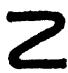
\includegraphics[keepaspectratio]{images/part002_ebf593f8.jpg}}

It is important to notice that if the series defined by a sequence \((x_{n})_{n\in \mathbb{N}}\) converges, there can exist infinite subsets I of \(\mathbf{N}\) such that the series defined by the subsequence \((x_{n})_{n\in \mathbb{I}}\) does not converge (see Exercise 5 and Chapter IV, § 7).

Propositions 4 and 5 extend immediately to series, and we leave their formulation in this case to the reader.

PROPOSITION 8 (Restricted associativity of series). Let \((k_n)\) be a strictly increasing sequence of integers \(\geqslant 0\) . If the series whose general term is \(x_n\) converges, and if we put \(u_n = \sum_{p=k_{n-1}}^{k_n-1} x_p\) , then the series whose general term is \(u_n\) is convergent, and we have \(\sum_{n=0}^{\infty} u_n = \sum_{n=0}^{\infty} x_n\) .

For the sequence of partial sums of the series \((u_{n})\) is a subsequence \((s_{k_{n}-1})\) of the sequence \((s_{n})\) of partial sums of the series \((x_{n})\) .

\subsection{COMMUTATIVELY CONVERGENT SERIES}

Let \((x_{n})\) be a summable sequence in \(G\) , and let \(s = \sum_{n\in \mathbb{N}}x_n\) be its sum. Then for each neighbourhood \(V\) of \(0\) , there exists \(J_0\in \mathfrak{F}(N)\) such that \(s_J\in s + V\) whenever \(J\in \mathfrak{F}(N)\) and \(J_0\subset J\) . Let \(m\) be the largest integer in \(J_0\) ; then if \(n\geqslant m\) we have \(s_n\in s + V\) , and therefore the series \((x_{n})\) is convergent and its sum is \(s\) . But the converse is false:

the sequence of terms of a convergent series can very well fail to be summable (see Chapter IV, § 7).

Moreover, the definition of a convergent series essentially involves the order structure of N. If the series \((x_{n})\) is convergent, and if \(\sigma\) is a permutation of N, then the series \((x_{\sigma(n)})\) is not necessarily convergent (cf.~Chapter IV, § 7, Exercise 15).

DEFINITION 2. A series defined by a sequence \((x_{n})\) is said to be commutatively convergent if, for each permutation \(\sigma\) of \(\mathbf{N}\) , the series defined by the sequence \((x_{\sigma(n)})\) is convergent.

PROPOSITION 9. The series defined by the sequence \((x_{n})\) is commutatively convergent if and only if the sequence \((x_{n})\) is summable; and then, for each permutation \(\sigma\) of \(\mathbf{N}\) , we have

\[
\sum_ {n = 0} ^ {\infty} x _ {\sigma} = \sum_ {n \in \mathbb {N}} x _ {n}.
\]

If the sequence is summable, then clearly the series is commutatively convergent. To prove the reverse implication we shall argue by reductio ad absurdum and suppose that the series \((x_{n})\) is commutatively convergent but that the sequence \((x_{n})\) is not summable. The image of the filter \(\Phi\) under the mapping \(\mathbf{H} \to s_{\mathbf{H}}\) therefore cannot be a Cauchy filter base in \(\mathbf{G}\) , otherwise this filter base would converge, since by hypothesis it has a cluster point (Chapter II, § 3, no. 2, Proposition 5, Corollary 2). Hence there is a neighbourhood \(\mathbf{V}\) of \(o\) in \(\mathbf{G}\) such that, for each finite subset \(\mathbf{J}\) of \(\mathbf{N}\) , there is a finite subset \(\mathbf{H}\) of \(\mathbf{N}\) which does not meet \(\mathbf{J}\) and is such that \(\sum_{n \in \mathbf{H}} x_{n} \notin V\) . Hence, by induction, we can define a partition of

N into finite subsets \(H_{k}\) ( \(k \in N\) ) such that \(\sum_{n \in H_{k}} x_{n} \notin V\) for an infinite number of indices k. Clearly there is a permutation \(\sigma\) of N such that for each k, the values of n for which \(\sigma(n) \in H_{k}\) are consecutive. If \(\sigma\) is such a permutation, then the series whose general term is \(x_{\sigma(n)}\) cannot be convergent, and we have a contradiction.

If the group G is written multiplicatively, the infinite product defined by a sequence \((x_{n})\) of points of G (or infinite product whose general term is \(x_{n}\) , or even product \(x_{n}\) if there is no possibility of confusion) is defined to be the pair formed by the sequence \((x_{n})\) and the sequence of partial products \(p_{n}=\prod_{k=0}^{n}x_{k}\) . The infinite product is said to converge if the sequence \((p_{n})\) converges, and the limit of this sequence is denoted by \(\prod_{n=0}^{\infty}x_{n}\) (or \(\prod_{n=0}^{\infty}x_{n}\) by abuse of notation). We leave to the reader the task of transcribing into multiplicative notation the properties of series which we have established.

\section{TOPOLOGICAL GROUPS WITH OPERATORS; TOPOLOGICAL RINGS, DIVISION RINGS AND FIELDS}

\subsection{TOPOLOGICAL GROUPS WITH OPERATORS}

On a set G, a structure of a group with operators and a topology are said to be compatible if the topology and the group structure of G are compatible (§ 1, no. 1) and if in addition the endomorphisms of G produced by the operators are continuous. The set G, together with the given topology and structure of group with operators, is then said to be a topological group with operators.

If H is a stable subgroup of a topological group G with operators, then the topology induced on H by the topology of G is compatible with the structure of group with operators on H. Furthermore:

PROPOSITION I. If H is a stable subgroup of a topological group G with operators, then the closure \(\overline{H}\) of H in G is a stable subgroup of G.

We know already (§ 2, no. 1, Proposition 1) that \(\overline{\mathbf{H}}\) is a subgroup of G. Also if \(\alpha\) is any operator on G, the image of H under the continuous mapping \(x \to x^{\alpha}\) is contained in H, and therefore the image of \(\overline{\mathbf{H}}\) is contained in \(\overline{\mathbf{H}}\) (Chapter I, § 2, no. 1, Theorem 1).

Let H be a stable normal subgroup of a topological group G with operators. Then for each operator \(\alpha\) on G, the mapping of G/H into itself induced by \(x \rightarrow x^{\alpha}\) is continuous (§ 2, no. 8, Remark 3), and the structure of group with operators on G/H is therefore compatible with the quotient topology on G/H.

Let \((\mathbf{G}_i)_{i\in I}\) be a family of topological groups with operators, where each \(\mathbf{G}_i\) is assumed to have the same operator set \(\Omega\) . For each \(\alpha \in \Omega\) , the mapping \(x\to ((\mathrm{pr}_i x)^{\alpha})\) of \(\mathbf{G} = \prod_{i\in I}\mathbf{G}_i\) into itself is continuous (Chapter I, § 4, no. 1, Proposition 1), and the structure of groups with operators on \(\mathbf{G}\) is therefore compatible with the product topology on \(\mathbf{G}\) .

If G is a Hausdorff topological group with operators and if G has a completion \(\hat{G}\) (§ 3, no. 4), then every endomorphism \(x \to x^{\alpha}\) of G defined by an operator on G can be extended by continuity to an endomorphism of \(\hat{\mathbf{G}}\) (§ 3, no. 3, Proposition 5). Hence \(\hat{\mathbf{G}}\) has the structure of a topological group with operators, and the operator set is the same for \(\hat{\mathbf{G}}\) as for \(\mathbf{G}\) .

\subsection{TOPOLOGICAL DIRECT SUM OF STABLE SUBGROUPS}

Since the study of commutative groups with operators is equivalent to the study of modules we shall sometimes allow ourselves to use the terminology proper to modules for arbitrary commutative groups with operators; thus we may speak of linear mappings instead of homomorphisms of commutative groups with operators, and we may use the word projector to denote an idempotent endomorphism of a commutative group with operators.

If a commutative topological group \(\mathbf{E}\) with operators (written additively) is the direct sum of a finite family \((\mathbf{M}_i)_{1 \leqslant i \leqslant n}\) of stable subgroups, then the canonical bijection \((x_i) \to \sum_{i=1}^{n} x_i\) of the product group \(\prod_{i=1}^{n} \mathbf{M}_i\) onto \(\mathbf{E}\) is continuous, but is not necessarily a homeomorphism.

DEFINITION 1. Let E be a commutative topological group with operators, and let \((\mathbf{M}_i)_{1 \leqslant i \leqslant n}\) be a finite family of stable subgroups of E, such that E is the direct sum of the \(\mathbf{M}_i\) . Then E is said to be the topological direct sum of the \(\mathbf{M}_i\) if the canonical mapping \((x_i) \to \sum_{i=1}^{n} x_i\) of the product group \(\prod_{i=1}^{n} \mathbf{M}_i\) onto E is a homeomorphism (and therefore an isomorphism of topological groups with operators).

PROPOSITION 2. Let E be a commutative topological group with operators which is the direct sum of stable subgroups \(\mathbf{M}_i\) ( \(1 \leqslant i \leqslant n\) ). Let \((p_i)_{1 \leqslant i \leqslant n}\) be the family of projectors associated with the decomposition \(\mathbf{E} = \sum_{i=1}^{n} \mathbf{M}_i\) . Then E is the topological direct sum of the \(\mathbf{M}_i\) if and only if the \(p_i\) are continuous.

For the mapping \(x \to (p_i(x))\) is the inverse of the mapping \((x_i) \to \sum_{i=1}^{n} x_i\) .

Since \(\mathbf{I} = \sum_{i=1}^{n} p_i\) (where \(\mathbf{I}\) denotes the identity mapping of \(\mathbf{E}\) ) it is sufficient for \(n - \mathbf{I}\) of the projectors \(p_i\) to be continuous in order that the \(n\) th should also be continuous.

If E is the topological direct sum of two stable subgroups M, N, then N is said to be a topological complement of M in E; this is the case if and only if the canonical mapping of E/M onto N is an isomorphism of topological groups with operators.

COROLLARY. Let E be a commutative topological group with operators, and let M be a stable subgroup of E. Then the following conditions are equivalent:

\begin{enumerate}
\def\labelenumi{\alph{enumi})}
\item
  M has a topological complement in E.
\item
  There is a continuous projector \(p\) of \(\mathbf{E}\) into \(\mathbf{E}\) such that \(p(\mathbf{E}) = \mathbf{M}\) .
\item
  The identity mapping of M can be extended to a continuous linear mapping of E onto M.
\end{enumerate}

It follows from Proposition 2 that a) implies b), and it is clear that b) implies c). Finally, if p is a continuous linear mapping of E onto M which extends the identity mapping of M, then p is a continuous projector, and the projectors p and 1-p are associated with the direct sum decomposition \(E = M + N\) , where \(N = p^{-1}(\mathbf{o})\) .

Remarks. 1) To avoid confusion, we shall sometimes say that a stable subgroup of E which is a complement of M (in the sense of the structure of group with operators, without a topology) is an algebraic complement of M.

\begin{enumerate}
\def\labelenumi{\arabic{enumi})}
\setcounter{enumi}{1}
\tightlist
\item
  If a Hausdorff commutative topological group with operators is the topological direct sum of a family \((\mathbf{M}_i)_{1\leqslant i\leqslant n}\) of stable subgroups, then each of the subgroups \(\mathbf{M}_i\) is closed in E, for \(\mathbf{M}_i\) is the set of all \(x\in E\) such that \(p_i(x) = x\) (Chapter I, § 8, no. 1, Proposition 2).
\end{enumerate}

PROPOSITION 3. Let E, F be two commutative topological groups with operators, and let u be a continuous linear mapping of E into F. In order that there should exist a continuous linear mapping v of F into E such that \(u \circ v\) is the identity mapping of F (in which case u is said to be right invertible and v is said to be a right inverse of u) it is necessary and sufficient that u is a strict morphism (§ 2, no. 8) of E onto F and that \(u^{-1}(\mathbf{o})\) has a topological complement in E.

The conditions are necessary. For we have then \(u(v(\mathbf{F})) = \mathbf{F}\) and \(a\) fortiori \(u(\mathbf{E}) = \mathbf{F}\) ; furthermore, if \(p = v \circ u\) , then \(p\) is a continuous linear mapping of \(\mathbf{E}\) into itself such that \(p^2 = p\) ; therefore (Corollary to Proposition 2) \(p(\mathbf{E}) = v(u(\mathbf{E})) = v(\mathbf{F})\) has a topological complement \(p^{-1}(\mathbf{o})\) in \(\mathbf{E}\) ; but since \(u(p(x)) = u(x)\) by hypothesis, we have \(u^{-1}(\mathbf{o}) = p^{-1}(\mathbf{o})\) . Finally, the bijective mapping of \(\mathrm{E}/p^{-1}(\mathbf{o})\) onto \(\mathbf{F}\) , associated with \(u\) , is the composition of the bijective mapping of \(\mathrm{E}/u^{-1}(\mathbf{o})\) onto \(v(\mathbf{F})\) , associated with \(p\) , and the restriction of \(u\) to \(v(\mathbf{F})\) ; since \(v\) is continuous, both these mappings are isomorphisms, and therefore \(u\) is a strict morphism of \(\mathbf{E}\) onto \(\mathbf{F}\) .

The conditions are sufficient. For if \(\varphi\) is the canonical homomorphism of E onto \(\mathrm{E}/u^{-1}(\mathbf{o})\) , to say that \(u^{-1}(\mathbf{o})\) has a topological complement M in E is to say that the restriction of \(\varphi\) to M is an isomorphism of M onto \(\mathrm{E}/u^{-1}(\mathbf{o})\) . Since on the other hand \(u=w\circ\varphi\) , where w is an isomorphism of \(\mathrm{E}/u^{-1}(\mathbf{o})\) onto F, we see that the restriction of u to M is an isomorphism of M onto F, and the inverse isomorphism v is therefore such that \(u\circ v\) is the identity mapping of F onto itself.

PROPOSITION 4. Let E, F be two commutative topological groups with operators, and let u be a continuous linear mapping of E into F. In order that there should exist a continuous linear mapping v of F into E such that \(v \circ u\) is the identity mapping of E onto itself (in which case u is said to be left invertible and v is said to be a left inverse of u) it is necessary and sufficient that u is a (topological) isomorphism of E onto u(E), and that u(E) has a topological complement in F.

The conditions are sufficient, for if they are satisfied we obtain a left inverse \(v\) of \(u\) by taking the composition of the isomorphism of \(u(\mathbf{E})\) onto \(\mathbf{E}\) which is the inverse of \(u\) , with a continuous projector of \(\mathbf{F}\) onto \(u(\mathbf{E})\) .

The conditions are necessary. For the relation \(v(u(x)) = x\) shows that \(u^{-1}(\mathbf{o}) = \{0\}\) ; \(u\) is therefore a bijection of \(E\) onto \(u(E)\) , and since the restriction of \(v\) to \(u(E)\) is continuous, it follows that \(u\) is an isomorphism of \(E\) onto \(u(E)\) . On the other hand, if we put \(q = u \circ v\) , then \(q\) is a continuous linear mapping of \(F\) onto \(u(E)\) such that \(q^2 = q\) , which proves (Corollary to Proposition 2) that \(u(E)\) has a topological complement in \(F\) .

\subsection{TOPOLOGICAL RINGS}

DEFINITION 2. A topological ring is a set A which carries a ring structure and a topology satisfying the following axioms:

\((\mathrm{AT}_{\mathbf{I}})\) . The mapping \((x,y) \to x + y\) of \(\mathbf{A} \times \mathbf{A}\) into \(\mathbf{A}\) is continuous.

\((\mathrm{AT}_{\mathbf{II}})\) . The mapping \(x \to -x\) of A into A is continuous.

\((\mathrm{AT}_{\mathrm{III}})\) . The mapping \((x,y)\to xy\) of \(\mathbf{A}\times \mathbf{A}\) into \(\mathbf{A}\) is continuous.

The first two axioms express that the topology of \(\mathbf{A}\) is compatible with its additive group structure (§ 1, no. 1).

If a ring structure and a topology are given on a set A, they are said to be compatible if they satisfy axioms \((\mathrm{AT}_{\mathbf{I}})\) , \((\mathrm{AT}_{\mathbf{II}})\) and \((\mathrm{AT}_{\mathbf{III}})\) .

Examples. 1) On any ring A, the discrete topology is compatible with the ring structure. A topological ring whose topology is discrete is called a discrete ring.

* 2) We shall see in Chapter IV that the topology of the rational line Q (resp. the real line R) is compatible with the ring structure of Q (resp. R). *

In a topological ring every left homothety \(x \rightarrow ax\) (resp. every right homothety \(x \rightarrow xa\) ) is continuous (and is a homeomorphism if a is a unit of A).

Since we can write identically

\[
x y - x _ {0} y _ {0} = (x - x _ {0}) (y - y _ {0}) + (x - x _ {0}) y _ {0} + x _ {0} (y - y _ {0})
\]

the axiom \((\mathrm{AT}_{\mathrm{III}})\) {[}in view of \((\mathrm{AT}_{\mathrm{I}})\) and \((\mathrm{AT}_{\mathrm{II}})\) {]} is equivalent to the conjunction of the following two axioms:

\((\mathrm{AT}_{\mathrm{III}a})\) . Given any \(x_0\in \mathbf{A}\) , the mappings \(x\to x_0x\) and \(x\rightarrow xx_0\) are continuous at the point \(x = 0\)

\((\mathrm{AT}_{\mathbf{III}\ b})\) . The mapping \((x,y)\rightarrow xy\) of \(\mathbf{A}\times \mathbf{A}\) into A is continuous at the point (o, o).

From this we can deduce a necessary and sufficient set of conditions which the filter \(\mathfrak{B}\) of neighbourhoods of \(o\) in a ring \(A\) must satisfy in order to define a topology on \(A\) compatible with its ring structure: \(\mathfrak{B}\) must satisfy axioms \((\mathrm{GA}_{\mathrm{I}})\) and \((\mathrm{GA}_{\mathrm{II}})\) of § 1, and also the following two axioms:

\((\mathrm{AV}_{1})\) . For all \(x_0\in \mathbf{A}\) and all \(\mathbf{V}\in \mathfrak{B}\) , there exists \(\mathbf{W}\in \mathfrak{B}\) such that \(x_0\mathbf{W}\subset \mathbf{V}\) and \(\mathbf{W}x_0\subset \mathbf{V}\)

\((\mathrm{AV}_{\mathrm{II}})\) . For all \(\mathbf{V} \in \mathfrak{B}\) , there exists \(\mathbf{W} \in \mathfrak{B}\) such that \(\mathbf{WW} \subset \mathbf{V}\) .

Remark. In analysis one fairly often meets rings which satisfy axioms \((\mathrm{AT}_{\mathrm{I}})\) , \((\mathrm{AT}_{\mathrm{II}})\) and \((\mathrm{AT}_{\mathrm{III}a})\) , but not \((\mathrm{AT}_{\mathrm{III}b})\) . * An example is the ring of measures on a compact group, where multiplication is convolution and the topology is the vague topology. *

Example 3). Let \(\mathfrak{B}\) be a filter base on a ring A, consisting of two-sided ideals. \(\mathfrak{B}\) is a fundamental system of neighbourhoods of o for a topology compatible with the additive group structure of A, and it follows immediately from \((\mathrm{AV}_{\mathrm{I}})\) and \((\mathrm{AV}_{\mathrm{II}})\) that this topology is compatible with the ring structure of A.

Let X be a topological space, and let f and g be two mappings of X into a topological ring A. If f and g are continuous at a point \(x_{0} \in X\) , then \(f + g\) , -f and fg are continuous at this point. It follows that the continuous mappings of X into A form a subring of the ring \(A^{X}\) of all mappings of X into A. We see also that, if A is commutative, then every polynomial in n variables, with coefficients in A and defined on \(A^{n}\) , is continuous on \(A^{n}\) . Again, let f and g be two mappings of a set X, filtered by a filter F, into a Hausdorff topological ring A; if \(\lim_{\mathfrak{F}} f\) and \(\lim_{\mathfrak{F}} g\) exist, then so do \(\lim_{\mathfrak{F}} (f + g)\) , \(\lim_{\mathfrak{F}} (-f)\) and \(\lim_{\mathfrak{F}} (fg)\) , and we have (Chapter I, §7, no. 4, Proposition 9, Corollary 1, and §8, no. 1, Proposition 1)

\[
\lim _ {\mathfrak {F}} (f + g) = \lim _ {\mathfrak {F}} f + \lim _ {\mathfrak {F}} g,\tag{1}
\]

\[
\lim _ {\mathfrak {F}} (- f) = - \lim _ {\mathfrak {F}} f,\tag{2}
\]

\[
\lim _ {\mathfrak {F}} (f g) = (\lim _ {\mathfrak {F}} f) (\lim _ {\mathfrak {F}} g).\tag{3}
\]

\subsection{SUBRINGS; IDEALS; QUOTIENT RINGS; PRODUCTS OF RINGS}

If H is a subring of a topological ring A, then the topology induced on H by that of A is compatible with the ring structure of H. The topological ring structure thus defined on H is said to be induced by that of A.

PROPOSITION 5. Let H be a dense subring of a topological ring A, and let K be a subring (resp. left ideal, right ideal, two-sided ideal) of H. Then the closure K of K in A is a subring (resp. left ideal, right ideal, two-sided ideal) of A.

The proof is the same as for Proposition 8 of § 2, n.~3: if for example K is a left ideal in H, then the mapping \((z, x) \to zx\) is continuous on \(A \times A\) and maps \(H \times K\) into K; hence it maps \(A \times K = \overline{H} \times K\) into \(\overline{H}\) .

Let H be a two-sided ideal in a topological ring A. By the same argument as for quotient groups, we see that the quotient of the topology of A by the relation \(x - y \in H\) is compatible with the ring structure of A/H. In particular, if A is not Hausdorff, then the closure N of \(\{o\}\) in A is a closed two-sided ideal, by Proposition 5; the quotient ring, which is Hausdorff (§ 2, no. 5, Proposition 13) is called the Hausdorff ring associated with A.

Let \((\mathbf{A}_t)_{t\in \mathbf{I}}\) be a family of topological rings. On the set \(\mathbf{A} = \prod_{t\in \mathbf{I}}\mathbf{A}_t\) , the product of the topologies of the \(\mathbf{A}_t\) is compatible with the product of the ring structures of the \(\mathbf{A}_t\) (same proof as for product groups); the topological ring \(\mathbf{A}\) thus defined is called the product of the topological rings \(\mathbf{A}_t\) .

\subsection{COMPLETION OF A TOPOLOGICAL RING}

When we speak of the uniformity of a topological ring, we always mean the uniformity of its additive group, unless the contrary is expressly stated; in particular, A is said to be a complete ring if the additive group of A is complete.

Let A be a Hausdorff topological ring; as an additive group A can be considered as a dense subgroup of a complete Hausdorff commutative group \(\hat{\mathbf{A}}\) , which is determined up to isomorphism (§ 3, no. 5, Theorem 2). In order that we should be able to consider A as a subring of a complete ring, it is necessary to be able to extend the function \(xy\) by continuity to the space \(\hat{\mathbf{A}} \times \hat{\mathbf{A}}\) . The possibility of this extension will follow from the following more general theorem:

THEOREM 1. Let E, F, G be three complete Hausdorff commutative groups; let A be a dense subgroup of E and let B be a dense subgroup of F. If f is a Z continuous Z-bilinear (*) mapping of A × B into G, then f can be extended by continuity to a continuous Z-bilinear mapping of E × F into G.

Let \((x_{0}, y_{0})\) be an arbitrary point of \(E \times F\) , and let \(\mathfrak{U}\) , \(\mathfrak{B}\) be the traces on A, B respectively of the neighbourhood filters of \(x_{0}, y_{0}\) ( \(\mathfrak{U}\) , \(\mathfrak{B}\) are filters, by hypothesis). To show that f can be extended by continuity, it is enough to show that \(f(\mathfrak{U} \times \mathfrak{V})\) is a Cauchy filter-base on G (Chapter II, § 3, no. 6, Proposition 11). Consider the identity

\[
f \left(x ^ {\prime}, y ^ {\prime}\right) - f (x, y) = f \left(x ^ {\prime} - x, y _ {1}\right) + f \left(x _ {1}, y ^ {\prime} - y\right) + f \left(x ^ {\prime} - x, y ^ {\prime} - y _ {1}\right).
\]

We shall show that by taking \((x, y)\) and \((x', y')\) in a sufficiently small set of \(\mathfrak{U} \times \mathfrak{B}\) , and by choosing \(x_{1}\) and \(y_{1}\) suitably, we can make each of the terms on the right-hand side very small. Let W be any neighbourhood of o in G; since f is continuous at \((o, o) \in A \times B\) , there is a set \(U \in \mathfrak{U}\) and a set \(V \in \mathfrak{B}\) such that \(f(x' - x, y' - y) \in W\) whenever \(x \in U\) , \(x' \in U\) , \(y \in V\) , \(y' \in V\) . Take a point \(x_{1} \in U\) and a point \(y_{1} \in V\) ; then for all \(x, x'\) in U and all \(y, y'\) in V we shall have

\[
f \left(x ^ {\prime} - x, y ^ {\prime} - y _ {1}\right) + f \left(x - x _ {1}, y ^ {\prime} - y\right) \in \mathrm{W} + \mathrm{W}.
\]

On the other hand, the partial mapping \(x \to f(x, y_1)\) is continuous on A; hence there is a set \(U' \subset U\) , belonging to \(\mathfrak{U}\) , and such that, whenever \(x\) and \(x'\) belong to \(U'\) , we have \(f(x' - x, y_1) \in W\) . Likewise there exists \(V' \subset V\) belonging to \(\mathfrak{B}\) such that, whenever \(y\) and \(y'\) belong to \(V'\) , we have \(f(x_1, y' - y) \in W\) . Consequently, if \((x, y)\) and \((x', y')\) are any two points of \(U' \times V'\) , then

\[
f \left(x ^ {\prime}, y ^ {\prime}\right) - f (x, y) \in W + W + W + W;
\]

this proves the existence of the extension \(\overline{f}\) of \(f\) . The fact that \(\overline{f}\) is \(\mathbf{Z}\) -bilinear is an immediate consequence of the principle of extension of identities (Chapter I, § 8, no. 1, Corollary 1 to Proposition 2).

Q.E.D.

In the application of this theorem to a Hausdorff topological ring A, we take E, F and G to be \(\hat{A}\) , A and B to be the ring A, and f to be the Z-bilinear mapping \((x, y) \to xy\) , which by hypothesis is continuous. We denote again by xy the value of the extended function on \(\hat{A} \times \hat{A}\) ; this function is a law of composition on \(\hat{A}\) , and to say that it is Z-bilinear means that it is distributive on both sides with respect to addition; and it is also associative, by the principle of extension of identities. Consequently:

PROPOSITION 6. A Hausdorff topological ring A is isomorphic to a dense subring of a complete Hausdorff ring \(\hat{\mathbf{A}}\) , which is determined up to isomorphism (and is called the completion of A).

If A is commutative (resp. has an identity element) then the same is true of \(\hat{A}\) (principle of extension of identities).

Let A be a topological ring, not necessarily Hausdorff; let N be the closure of \(\{o\}\) in A, and let \(A' = A/N\) be the Hausdorff ring associated with A. Then \(\hat{A}'\) , the completion of \(A'\) , is called the Hausdorff completion of A and is also denoted by \(\hat{A}\) . One shows as in §3, no. 4, Proposition 8 that every continuous ring homomorphism u of A with a complete Hausdorff topological ring C can be uniquely factorized as \(u = v \circ \varphi\) , where v is a continuous homomorphism of \(\hat{A}\) into C and \(\varphi\) is the canonical mapping of A into \(\hat{A}\) . If A, B are two topological rings, and \(u : A \to B\) is a continuous homomorphism, there is therefore a unique continuous homomorphism \(\hat{u} : \hat{A} \to \hat{B}\) such that the diagram

\[
\begin{array}{c c c} \mathbf {A} & \stackrel {{u}} {{\longrightarrow}} & \mathbf {B} \\ \varphi \Big \downarrow & & \Big \downarrow \psi \\ \hat {\mathbf {A}} & \stackrel {{\hat {u}}} {{\longrightarrow}} & \hat {\mathbf {B}} \end{array}
\]

is commutative ( \(\varphi\) and \(\psi\) being the canonical mappings); we have only to apply the preceding result to \(\psi \circ u\) .

\subsection{TOPOLOGICAL MODULES}

DEFINITION 3. Given a topological ring A with an identity element, a topological left A-module is a set E, together with:

\begin{enumerate}
\def\labelenumi{\arabic{enumi})}
\item
  a left A-module structure;
\item
  a topology compatible with the additive group structure of E, and satisfying the following axiom:
\end{enumerate}

(MT) The mapping \((\lambda, x) \to \lambda x\) of \(\mathbf{A} \times \mathbf{E}\) into \(\mathbf{E}\) is continuous.

We define similarly the notion of a topological right A-module; since every right A-module can be considered as a left A°-module, where A° is the opposite ring of A, and since the topology of A is compatible with the ring structure of A°, there is no need to distinguish between topological right A-modules and topological left A°-modules.

Examples. *1) A topological vector space over R (resp. C) is a topological R (resp. C) module.

\begin{enumerate}
\def\labelenumi{\arabic{enumi})}
\setcounter{enumi}{1}
\tightlist
\item
  Let A be a ring and let B be a filter base on A consisting of two-sided ideals of A; let E be a left A-module. If we give A the topology (compatible with its ring structure) for which B is a fundamental system of neighbourhoods of o (no. 3, Example 3), and E the topology (compatible with its additive group structure) in which the sets aE, as a runs through B, form a fundamental system of neighbourhoods of o (§ 1, no. 2, Example), it is immediately verified that E is a topological A-module.
\end{enumerate}

Remark. Given a topological ring A, consider, on a left A-module E, a topology compatible with the additive group structure of E. By virtue of the identity

\[
\lambda x - \lambda_ {0} x _ {0} = (\lambda - \lambda_ {0}) x _ {0} + \lambda_ {0} (x - x _ {0}) + (\lambda - \lambda_ {0}) (x - x _ {0})
\]

the axiom (MT) is equivalent to the conjunction of the following three axioms:

\((\mathbf{MT}_{\mathbf{I}}^{\prime})\) . For each \(x_0\in \mathbf{E}\) , the mapping \(\lambda \to \lambda x_0\) is continuous at the point \(\lambda = 0\)

\((\mathbf{MT}_{\mathrm{II}}^{\prime})\) . For each \(\lambda_0\in \mathbf{A}\) , the mapping \(x\to \lambda_0x\) is continuous at the point \(x = 0\)

\((\mathbf{MT}_{\mathrm{III}}^{\prime})\) . The mapping \((\lambda ,x)\to \lambda x\) is continuous at the point (o, o).

We deduce from this a necessary and sufficient set of conditions that the filter \(\mathfrak{B}\) of neighbourhoods of o in an A-module E must satisfy in order to define a topology on E compatible with its module structure; \(\mathfrak{B}\) must satisfy the axioms (GA \(_{\mathrm{I}}\) ) and (GA \(_{\mathrm{II}}\) ) of § 1, no. 2, and in addition must satisfy the following three axioms:

\((\mathbf{MV}_{\mathrm{I}})\). For each \(x_0 \in E\) and V \(\in \mathfrak{B}\) , there is a neighbourhood S of o in A such that S. \(x_0 \subset V\) .

\((\mathbf{MV}_{\mathrm{II}})\) . For each \(\lambda_0 \in \mathbf{A}\) and \(V \in \mathfrak{B}\) , there exists \(W \in \mathfrak{B}\) such that \(\lambda_0 W \subset V\) . \((\mathbf{MV}_{\mathrm{III}})\) . For each \(V \in \mathfrak{B}\) there exists \(U \in \mathfrak{B}\) and a neighbourhood \(T\) of \(o\) in \(A\) such that \(T. U \subset V\) .

Every commutative topological group is a topological \(\mathbf{Z}\) -module when the ring \(\mathbf{Z}\) is given the discrete topology.

If M is a submodule of a topological A-module E, it is clear that the topology induced on M by the topology of E is compatible with the module structure of M. Moreover, on the quotient A-module E/M, the topology which is the quotient by M of the topology of E is compatible with the A-module structure. To see this it is enough to show that the mapping \((\lambda, \dot{x}) \to \lambda \dot{x}\) of \(\mathbf{A} \times (\mathbf{E} / \mathbf{M})\) onto \(\mathbf{E} / \mathbf{M}\) is continuous (where \(x \to \dot{x}\) denotes the canonical mapping of \(\mathbf{E}\) onto \(\mathbf{E} / \mathbf{M}\) ). Now, since we may identify the additive topological groups \(\mathbf{A} \times (\mathbf{E} / \mathbf{M})\) and \((\mathbf{A} \times \mathbf{E}) / (\{\mathbf{o}\} \times \mathbf{M})\) (§ 2, no. 9, Corollary to Proposition 26), it is enough to show that the mapping \((\lambda, x) \to \lambda \dot{x}\) of \(\mathbf{A} \times \mathbf{E}\) into \(\mathbf{E} / \mathbf{M}\) is continuous; and this is immediate, since the mapping in question is the composition of \(x \to \dot{x}\) and \((\lambda, x) \to \lambda x\) .

Let \((\mathbf{E}_i)_{i\in \mathbf{I}}\) be an arbitrary family of topological A-modules, and let \(\mathbf{E} = \prod_{i\in \mathbf{I}}\mathbf{E}_i\) be the A-module which is the product of the \(\mathbf{E}_i\) . Then the

product topology on E is compatible with the A-module structure of E. To prove this it is enough to show that the mapping \((\lambda, x) \to (\lambda \cdot \text{pr}_i x)_{i \in I}\) of A × E into E is continuous, or (by Proposition 1 of Chapter I, § 4, no. 1) that for each index \(i \in I\) the mapping \((\lambda, x) \to \lambda \cdot \text{pr}_i x\) is a continuous mapping of A × E into \(E_i\) ; but this mapping is the composition of \((\lambda, x_i) \to \lambda x_i\) and \((\lambda, x) \to (\lambda, \text{pr}_i x)\) , both of which are continuous.

Let A be a Hausdorff topological ring and E a Hausdorff topological A-module. Let \(\hat{\mathbf{E}}\) be the additive group which is the completion of the commutative topological group E (§ 3, no. 5, Theorem 2). The Z-bilinear mapping \((\lambda, x) \to \lambda x\) of the product \(\mathbf{A} \times \mathbf{E}\) of the additive groups A, E into the additive group E can be extended by continuity to a Z-bilinear mapping of \(\hat{\mathbf{A}} \times \hat{\mathbf{E}}\) into \(\hat{\mathbf{E}}\) (no. 5, Theorem 1), and this mapping we continue to denote by \((\lambda, x) \to \lambda x\) . By virtue of the principle of extension of identities, we have \(\lambda(\mu x) = (\lambda \mu)x\) for \(\lambda \in \hat{\mathbf{A}}\) , \(\mu \in \hat{\mathbf{A}}\) and \(x \in \hat{\mathbf{E}}\) , and \(1.x = x\) for all \(x \in \hat{\mathbf{E}}\) ; the external law \((\lambda, x) \to \lambda x\) therefore defines an \(\hat{\mathbf{A}}\) -module structure on \(\hat{\mathbf{E}}\) compatible with its topology. The topological \(\hat{\mathbf{A}}\) -module \(\hat{\mathbf{E}}\) thus defined is called the completion of the topological A-module E.

Let E be a topological module over a topological ring A, where neither A nor E is necessarily Hausdorff. Let N (resp. F) be the closure of \(\{o\}\) in A (resp. E). N is a two-sided ideal of A (no. 4, Proposition 5) and F is a sub-A-module of E (no. 1, Proposition 1); furthermore, by continuity we have \(\lambda x \in F\) whenever \(\lambda \in N\) or \(x \in F\) . We can therefore define, by passing to the quotients, a mapping \((\dot{\lambda}, \dot{x}) \to \dot{\lambda} \dot{x}\) of \((A/N) \times (E/F)\) into E/F; it is easily verified (by use of the Corollary to Proposition 26 of § 2, no. 9) that this mapping is continuous, and therefore defines a structure of a topological \((A/N)\) -module on E/F. If we put B = A/N and L = E/F, then the B-module L is called the Hausdorff module associated with E; its completion \(\hat{L}\) is a topological module over the Hausdorff completion \(\hat{A}\) (equal by definition to \(\hat{B}\) ) of A (no. 5), and this module \(\hat{L}\) is called the Hausdorff completion of E and is denoted

by \(\hat{\mathbf{E}}\) . We see as in § 3, no. 4, Proposition 8 that every continuous homomorphism \(u: \mathbf{E} \to \mathbf{G}\) of \(\mathbf{E}\) into a complete Hausdorff \(\hat{\mathbf{A}}\) -module \(\mathbf{G}\) factorizes uniquely into \(u = v \circ \varphi\) , where \(v\) is a continuous homomorphism of \(\hat{\mathbf{E}}\) into \(\mathbf{G}\) and \(\varphi\) is the canonical mapping of \(\mathbf{E}\) into \(\hat{\mathbf{E}}\) . We conclude that if \(\mathbf{E}, \mathbf{E}'\) are two topological A-modules and \(u: \mathbf{E} \to \mathbf{E}'\) is a continuous homomorphism, then there is a unique continuous homomorphism \(\hat{u}: \hat{\mathbf{E}} \to \hat{\mathbf{E}}'\) such that the diagram

\[
\begin{array}{c c c} \mathbf {E} & \stackrel {{u}} {{\longrightarrow}} & \mathbf {E} ^ {\prime} \\ \varphi \Big \downarrow & & \Big \downarrow \varphi^ {\prime} \\ \hat {\mathbf {E}} & \stackrel {{\hat {u}}} {{\longrightarrow}} & \hat {\mathbf {E}} ^ {\prime} \end{array}
\]

is commutative, \(\varphi\) and \(\varphi'\) being the canonical mappings.

The definitions and results of this section apply equally well to pseudo-modules over an arbitrary topological ring, by deleting all mention of the identity element of the ring.

\subsection{TOPOLOGICAL DIVISION RINGS AND FIELDS}

In what follows, and in Chapters IV and V, if K is a division ring we shall denote by \(K^{*}\) the multiplicative group of non-zero elements of K.

DEFINITION 4. A topological division ring is a set K carrying a division ring structure and a topology compatible with the ring structure of K, and satisfying in addition the following axiom:

(KT) The mapping \(x \to x^{-1}\) of \(\mathbf{K}^*\) into \(\mathbf{K}^*\) is continuous.

A commutative topological division ring is called a topological field.

A division ring structure and a topology on a set K are said to be compatible if the corresponding ring structure and the topology are compatible and if in addition axiom (KT) is satisfied.

Examples. 1) On any division ring K, the discrete topology is compatible with the division ring structure. A topological division ring whose topology is discrete is called a discrete division ring.

* 2) The topology of the rational line Q (resp. the real line R) is compatible with the field structure of R (resp. R) (see Chapter IV, § 3).*

Definition 4 shows that, if K is a topological division ring, then the topology induced by that of K on the multiplicative group \(K^{*}\) is compatible with the group structure of \(K^{*}\) .

If \(a \neq 0\) , the homotheties \(x \rightarrow ax\) and \(x \rightarrow xa\) are homeomorphisms of K onto itself; and so is the mapping \(x \rightarrow ax + b\) for all \(b \in K\) . Note that the homotheties \(x \rightarrow ax\) and \(x \rightarrow xa\) are automorphisms of the (topological) additive group of K if \(a \neq 0\) . If V is any neighbourhood of o in K, it follows therefore that aV and Va are neighbourhoods of o for all \(a \neq 0\) .

Let X be a topological space, and let f be a mapping of X into a topological division ring K. If f is continuous at a point \(x_{0} \in X\) and if \(f(x_{0}) \neq 0\) , then \(f^{-1}\) is continuous at \(x_{0}\) . In particular, if K is a topological field, then every rational function in n variables with coefficients in K is continuous at every point of \(K^{n}\) where its denominator does not vanish.

Likewise, if \(f\) is a mapping of a set \(\mathbf{X}\) , filtered by a filter \(\mathfrak{F}\) , into a Hausdorff topological division ring \(\mathbf{K}\) , and if \(\lim_{\mathfrak{F}} f\) exists and is not \(o\) , then \(\lim_{\mathfrak{F}} f^{-1}\) exists and we have

\[
\lim _ {\mathfrak {F}} f ^ {- 1} = (\lim _ {\mathfrak {F}} f) ^ {- 1}.\tag{4}
\]

If H is a division subring of a topological division ring K, then the topology induced on H by the topology of K is compatible with the division ring structure of H. The structure of a topological division ring thus defined on H is said to be induced by that of K. Furthermore, \(\overline{H}\) is also a division subring of K (the proof is analogous to that of Proposition 5).

In a topological division ring K, the closure of the set \(\{0\}\) is a two-sided ideal, by Proposition 5, and hence must be either \(\{0\}\) or K. In other words, if the topology of K is not the coarsest topology (Chapter I, § 2, no. 2) then it is Hausdorff (§ 1, no. 2, Proposition 2).

\subsection{UNIFORMITIES ON A TOPOLOGICAL DIVISION RING}

If K is a topological division ring it is necessary to distinguish between: 1) the uniformity of the additive group of K, which is defined on K and is called the additive uniformity of K; and 2) the left and right uniformities of the multiplicative group \(\mathbf{K}^*\) , which are defined on \(\mathbf{K}^*\) and are called (by abuse of language) the multiplicative uniformities of K.

The uniformity induced on \(K^{*}\) by the additive uniformity of K is in general distinct from the multiplicative uniformities of K (see Exercise 17).

By Proposition 6, a Hausdorff topological division ring K can be considered as a dense subring of a complete Hausdorff ring \(\hat{K}\) . In order that \(\hat{K}\) should be a topological division ring it is necessary that the mapping \(x \to x^{-1}\) be extendable by continuity to \((\hat{\mathbf{K}})^{*}\) ; and this necessary condition is also sufficient, for the functions \(xx^{-1}, x^{-1}x\) and \(1\) are then equal on \((\hat{\mathbf{K}})^{*}\) by reason of the principle of extension of identities, and therefore the value of the extended function is the inverse of \(x\) for each \(x \neq 0\) in \(\hat{\mathbf{K}}\) . In other words (cf.~Chapter II, § 3, no. 6, Proposition 11):

PROPOSITION 7. The completion \(\hat{\mathbf{K}}\) of a Hausdorff topological division ring \(\mathbf{K}\) is a topological division ring if and only if the image under the mapping \(x \to x^{-1}\) of every Cauchy filter (with respect to the additive structure) which does not have a cluster point at 0, is a Cauchy filter (with respect to the additive structure).

\pandocbounded{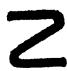
\includegraphics[keepaspectratio]{images/part002_56877e98.jpg}}

There are topological division rings in which this condition is not satisfied and in which the ring \(\hat{\mathbf{K}}\) has zero divisors (see Exercise 26). Moreover, even if the completion \(\hat{\mathbf{K}}\) is a topological division ring, there is no a priori reason to assume that the multiplicative structures of \(\hat{\mathbf{K}}\) are structures of a complete space. However, this will be the case for division rings \(\mathbf{K}\) such that \(\hat{\mathbf{K}}\) is locally compact (see Chapter I, § 9, no. 7, Proposition 13, and Chapter III, § 3, no. 3, Proposition 4) and for topological fields; for the latter, we have the following proposition:

PROPOSITION 8. If the additive uniform structure of a topological field K is a structure of a complete Hausdorff space, then the multiplicative structure on \(K^{*}\) is a structure of a complete space.

We shall show that if \(\mathfrak{F}\) is a Cauchy filter with respect to the multiplicative structure on \(\mathbf{K}^*\) , then \(\mathfrak{F}\) is a Cauchy filter with respect to the additive structure on \(\mathbf{K}\) , and does not converge to \(o\) ; this will establish the result. Let \(\mathbf{U}\) be any neighbourhood of \(o\) in \(\mathbf{K}\) , let \(\mathbf{V}\) be a closed neighbourhood of \(o\) such that \(\mathbf{V} \subset \mathbf{U}\) , \(\mathbf{VV} \subset \mathbf{U}\) {[}axiom \((\mathrm{AV}_{\mathrm{II}})]\) and \(-1 \notin V\) ; then by hypothesis there is a set \(\mathbf{A} \in \mathfrak{F}\) such that, for all \(x \in \mathbf{A}\) and \(y \in \mathbf{A}\) , we have \(x^{-1}y \in 1 + V\) . Let \(a \in \mathbf{A}\) , then \(\mathbf{A} \subset a + aV\) , and \(a + aV\) is a closed set which does not contain \(o\) ; hence \(o\) is not in the closure of \(\mathbf{A}\) and is therefore not a cluster point of \(\mathfrak{F}\) . Let \(\mathbf{W}\) be a neighbourhood of \(o\) such that \(aW \subset V\) {[}axiom \((\mathrm{AV}_{\mathrm{I}})]\) ; then by hypothesis there is a set \(\mathbf{B} \in \mathfrak{F}\) such that \(\mathbf{B} \subset \mathbf{A}\) and, for all \(x \in B\) and \(y \in B\) , we have \(x^{-1}y \in 1 + W\) ; hence \(y - x \in xW \subset AW \subset aW + aVW\) ; but \(\mathbf{K}\) is commutative, and therefore \(aVW = aWV \subset VV \subset U\) ; consequently \(y - x \in U + U\) and the Proposition is proved.

The same proof shows that Proposition 8 can be extended to the case in which every Cauchy filter with respect to one of the multiplicative structures of K is also a Cauchy filter with respect to the other multiplicative structure.

\section{INVERSE LIMITS OF TOPOLOGICAL GROUPS AND RINGS}

Throughout this section, I denotes a non-empty directed set (*) and \(\alpha \leqslant \beta\) denotes the partial order relation in I. Unless the contrary is expressly stated, all the inverse systems considered are indexed by I.
